% Copyright 2016 by Wang Kunzhen <wangkunzhen1993@gmail.com>.
%
% This is a latex template adapted from Till Tantau's Beamer template.
% It adds theme customizations for the convenience of users from the
% National University of Singapore. 
% 
% In principle, this file can be redistributed and/or modified under
% the terms of the GNU Public License, version 2.
%
% However, this file is supposed to be a template to be modified
% for your own needs. For this reason, if you use this file as a
% template and not specifically distribute it as part of a another
% package/program, I grant the extra permission to freely copy and
% modify this file as you see fit and even to delete this copyright
% notice. 

\documentclass[xcolor=dvipsnames]{beamer}

% There are many different themes available for Beamer. A comprehensive
% list with examples is given here:
% http://deic.uab.es/~iblanes/beamer_gallery/index_by_theme.html
% You can uncomment the themes below if you would like to use a different
% one:
%\usetheme{AnnArbor}
%\usetheme{Antibes}
%\usetheme{Bergen}
% \usetheme{Berkeley}
%\usetheme{Berlin}
%\usetheme{Boadilla}
% \usetheme{boxes}
%\usetheme{CambridgeUS}
%\usetheme{Copenhagen}
%\usetheme{Darmstadt}
%\usetheme{default}
\usetheme{Frankfurt}
%\usetheme{Goettingen}
%\usetheme{Hannover}
% \usetheme{Ilmenau}
% \usetheme{JuanLesPins}
% \usetheme{Luebeck}
% \usetheme{Madrid}
% \usetheme{Malmoe}
%\usetheme{Marburg}
% \usetheme{Montpellier}
% \usetheme{PaloAlto}
% \usetheme{Pittsburgh}
% \usetheme{Rochester}
% \usetheme{Singapore}
% \usetheme{Szeged}
% \usetheme{Warsaw}

\definecolor{nus-orange}{RGB}{239,124,0} 
\definecolor{nus-white}{RGB}{255,255,255}
\definecolor{nus-blue}{RGB}{0,61,124}
\definecolor{nus-black}{RGB}{0,0,0}

% Uncomment this section if you want the title background for each slide to be gradient like decaying from nus-orange to nus-white.
% \useoutertheme{shadow}
% \usepackage{tikz}
% \usetikzlibrary{shadings}
% \colorlet{titleleft}{nus-orange}
% \colorlet{titleright}{nus-orange!45!nus-white}
% \makeatletter
% \pgfdeclarehorizontalshading[titleleft,titleright]{beamer@frametitleshade}{\paperheight}{%
%   color(0pt)=(titleleft);
%   color(\paperwidth)=(titleright)}
% \makeatother
% End of gradient slide title effect.

\setbeamercolor{section in head/foot}{bg=nus-blue, fg=nus-white}
\setbeamercolor{subsection in head/foot}{bg=nus-blue, fg=nus-white}
\setbeamercolor{frametitle}{bg=nus-orange, fg=nus-white}
\setbeamercolor{title}{bg=nus-orange, fg=nus-white}
\setbeamercolor{alerted text}{fg=nus-orange}
\setbeamercolor{block title}{fg=nus-white}
\setbeamercolor{block body}{fg=nus-black}

\setbeamertemplate{theorems}[numbered]
\setbeamertemplate{propositions}[numbered]

\setbeamertemplate{bibliography item}{\insertbiblabel}

\setbeamertemplate{title page}[default][colsep=-4bp,rounded=true, shadow=true]

\usefonttheme[onlymath]{serif}
\setbeamertemplate{footline}[totalframenumber]

\addtobeamertemplate{navigation symbols}{}{
  \hspace{1em} \raisebox{1.35pt}{\usebeamerfont{footline}%
\insertframenumber/\inserttotalframenumber} }

\renewcommand\qedsymbol{$\blacksquare$}
% \setbeamertemplate{qed symbol}{$\blacksquare$}

\usepackage{braket}
\usepackage{multirow}
\usepackage{diagbox} % diagonal box in table
\usepackage{adjustbox} % allow tables to take up the space they need
\usepackage{graphicx} % allows figures to be inserted and scaled
\usepackage{listings} % allows for source code blocks
\usepackage{fancyvrb} % robust verbatim
\usepackage{fvextra} % robuster verbatim
\usepackage{siunitx} % allows SI units to be formatted
\usepackage{booktabs} % nice lines at top and bottom of tables

% \def\FancyVerbSpace{\textvisiblespace\kern0.07em}
% https://tex.stackexchange.com/questions/120207/customise-textvisiblespace
\newsavebox{\textvisiblespacebox}
\savebox{\textvisiblespacebox}{\texttt{a}}
\newcommand\vartextvisiblespace[1][\wd\textvisiblespacebox]{%
  \makebox[#1]{\kern.1em\rule{.4pt}{.3ex}%
  \hrulefill%
  \rule{.4pt}{.3ex}\kern.1em}%
}
\def\FancyVerbSpace{\vartextvisiblespace}


\usepackage[backend=biber, style=ieee-alphabetic]{biblatex}  
\addbibresource{../wiring.bib}
% \usepackage{hyperref} % hyperlinks
% \hypersetup{%
%   colorlinks=true,
%   linkcolor=purple,
%   urlcolor=blue
% }
\graphicspath{ {../images/} }

\newenvironment{Tabular}[1] % less cramped tables
{\def\arraystretch{1.75}\begin{tabular}{#1}}
{\end{tabular}}
\newenvironment{Array*}[1] % less cramped display mode arrays
{\def\arraystretch{1.75}\everymath={\displaystyle}\[\begin{array}{#1}}
{\end{array}\]}
\newenvironment{Array}[1] % less cramped display mode arrays
{\def\arraystretch{1.75}\everymath={\displaystyle}\begin{equation}\begin{array}{#1}}
{\end{array}\end{equation}}
\newenvironment{displaytable}[1] % environment for a simple inline table to present some information
{\vspace\abovedisplayskip\begin{center}\begin{tabular}{#1}}
{\end{tabular}\end{center}\vspace\belowdisplayskip}

\usepackage{mathtools}
\usepackage{tikz}
\usepackage{tikzscale} % include .tikz files with includegraphics and scale them
\usetikzlibrary{shapes, shapes.geometric, automata, positioning, arrows.meta, decorations.markings,decorations.pathreplacing, intersections, math, 3d, backgrounds}
\newcommand{\expandidx}[2]{%
  \expandafter#1\expandafter{\the\numexpr#2\relax}%
}

    \tikzset{%
      >={Stealth[width=4pt, length=6pt]}, % makes the arrow heads bold
      node distance=3cm, % specifies the minimum distance between two nodes. Change if necessary.
      % style to apply some styles to each segment of a path
      on each segment/.style={
        decorate,
        decoration={
          show path construction,
          moveto code={},
          lineto code={
            \path [#1]
            (\tikzinputsegmentfirst) -- (\tikzinputsegmentlast);
          },
          curveto code={
            \path [#1] (\tikzinputsegmentfirst)
            .. controls
            (\tikzinputsegmentsupporta) and (\tikzinputsegmentsupportb)
            ..
            (\tikzinputsegmentlast);
          },
          closepath code={
            \path [#1]
            (\tikzinputsegmentfirst) -- (\tikzinputsegmentlast);
          },
        },
      },
      set mid arrow/.code={\pgfqkeys{/tikz/mid arrow}{#1}},
      set mid arrow={pos/.initial=.5, end/.initial=stealth},
      mid arrow/.style={
        set mid arrow={#1},
        postaction={
          decorate,
          decoration={
            markings,
            mark=at position \pgfkeysvalueof{/tikz/mid arrow/pos}
                 with \arrow{\pgfkeysvalueof{/tikz/mid arrow/end}}
          }
        }
      },
      % simple black circle at node
      point/.style={circle,draw,inner sep=0pt,minimum size=3pt,fill=black},
      % nonclassical causation
      classbox/.style={rectangle, draw, line width=1pt},
      nclassbox/.style={rectangle, double, draw, rounded corners},
      classinfl/.style={-, line width=1pt},
      nclassinfl/.style={double},
      % coin with label and colours
      % TODO DOES NOT WORK
      set coin/.code={\pgfqkeys{/tikz/coin}{#1}},
      set coin={bg/.initial=black, fg/.initial=white},
      coin/.style={
        set coin={#1},
        postaction={
          circle,draw=\pgfkeysvalueof{/tikz/coin/fg},
          text=\pgfkeysvalueof{/tikz/coin/fg},
          fill=\pgfkeysvalueof{/tikz/coin/bg}
        }
      }
    }




\tikzset{%
  % simple black circle at node
  point/.style={circle,draw,inner sep=0pt,minimum size=3pt,fill=black},
  % coin with label and colours
  % TODO DOES NOT WORK
  set coin/.code={\pgfqkeys{/tikz/coin}{#1}},
  set coin={bg/.initial=black, fg/.initial=white},
  coin/.style={
    set coin={#1},
    postaction={
      circle,draw=\pgfkeysvalueof{/tikz/coin/fg},
      text=\pgfkeysvalueof{/tikz/coin/fg},
      fill=\pgfkeysvalueof{/tikz/coin/bg}
    }
  }
}

\RequirePackage{luatex85}
% Default preamble
\usepackage{pgfplots}
\pgfplotsset{compat=newest}
\usepgfplotslibrary{groupplots}
\usepgfplotslibrary{polar}
\usepgfplotslibrary{smithchart}
\usepgfplotslibrary{statistics}
\usepgfplotslibrary{dateplot}
\usepgfplotslibrary{ternary}
\usetikzlibrary{arrows.meta}
\usetikzlibrary{backgrounds}
\usepgfplotslibrary{patchplots}
\usepgfplotslibrary{fillbetween}
\pgfplotsset{%
  layers/standard/.define layer set={%
    background,axis background,axis grid,axis ticks,axis lines,axis tick labels,pre main,main,axis descriptions,axis foreground%
    }{grid style= {/pgfplots/on layer=axis grid},%
    tick style= {/pgfplots/on layer=axis ticks},%
    axis line style= {/pgfplots/on layer=axis lines},%
    label style= {/pgfplots/on layer=axis descriptions},%
    legend style= {/pgfplots/on layer=axis descriptions},%
    title style= {/pgfplots/on layer=axis descriptions},%
    colorbar style= {/pgfplots/on layer=axis descriptions},%
    ticklabel style= {/pgfplots/on layer=axis tick labels},%
    axis background@ style={/pgfplots/on layer=axis background},%
    3d box foreground style={/pgfplots/on layer=axis foreground},%
  },
}

    \usepackage{mleftright} % fix spacing issues in \left and \right
    \mleftright % rename left/right -> mleft/mright

    % analysis and calculus
    \DeclareMathOperator*{\argmin}{argmin}
    \DeclareMathOperator*{\argmax}{argmax}
    \newcommand{\norm}[1]{\mathop{}\left\lVert#1\right\rVert}
    \newcommand{\abs}[1]{\mathop{}\left\lvert#1\right\rvert}
    \newcommand{\indif}{{\mathop{}\!\mkern3mu\mathchar'26\mkern-12mu \mathrm{d}}}
    \newcommand{\Dif}{\mathop{}\!\mathrm{D}} % Difference operator
    \newcommand{\dif}{\mathop{}\!\mathrm{d}} % differential d
    \newcommand{\dintv}[2]{\mathopen\{#1,\ldots,#2\mathclose\}}
    \DeclarePairedDelimiterX{\ocintv}[2]{(}{]}{#1,#2}
    \DeclarePairedDelimiterX{\cointv}[2]{[}{)}{#1,#2}
    \DeclarePairedDelimiterX{\ccintv}[2]{[}{]}{#1,#2}
    \DeclarePairedDelimiterX{\oointv}[2]{(}{)}{#1,#2}

    % CS, discrete maths, algebra
    \DeclareMathSymbol{\lneg}{\mathord}{symbols}{"18} % tildes for negation
    \newcommand{\st}{\mathrel{:}} % 'such that'
    \newcommand{\?}{\mathrel{?}} % ternary operator
    \newcommand{\concat}{\mathbin{\Vert}} % string concatenation operator
    \newcommand{\Mod}{~\mathbf{mod}~} % for mod operator
    \newcommand{\Div}{~\mathbf{div}~} % for div operator
    \newcommand{\Rem}{~\mathbf{rem}~} % for rem operator
    \newcommand{\Z}{\mathbb{Z}} % for integers
    \newcommand{\R}{\mathbb{R}} % for reals
    \newcommand{\C}{\mathbb{C}} % for complex
    \newcommand{\ceil}[1]{\left\lceil#1\right\rceil} % enables \ceil{} for ceil delimiter
    \newcommand{\floor}[1]{\left\lfloor#1\right\rfloor} % enables \floor{} for floor delimiter

    % linear algebra
    \newcommand{\Lin}[1]{\mathbb{L}\left(#1\right)}
    \newcommand{\tpose}{\mathrm{T}}
    \newcommand{\cvec}[1]{\boldsymbol{\mathbf{#1}}}    % column vectors
    \newcommand{\rvec}[1]{\boldsymbol{\mathbf{#1}}^\tpose} % row vectors (transposed from column vectors)
    \newcommand{\bvec}[1]{\hat{\boldsymbol{\mathbf{#1}}}} % basis vectors
    \newcommand{\matr}[2][]{\left[\mathbf{#2}#1\right]} % matrices
    \newcommand{\inner}[2]{\left\langle#1,#2\right\rangle} % inner product
    % \newcommand{\dim}{\rm dim} % dimension

    % probability and statistics
    \newcommand{\rv}[1]{\boldsymbol{\mathbf{#1}}} % random variable
    \newcommand{\E}{\mathbb{E}} % expectation
    \newcommand{\angleb}[1]{\left\langle #1 \right\rangle} % physicist's notation for mean
    \newcommand{\Var}{\mathrm{Var}} % variance
    \newcommand{\indep}{\mathrel{\perp \!\!\! \perp}} % independence symbol
    \newcommand{\indic}[1]{\delta{\left\{#1\right\}}} % indicator function
    \newcommand*\markov{\mathrel{\ooalign{\hidewidth$\circ$\hidewidth\cr$-$\cr}}} % Markov chain

    % quantum physics
    \newcommand{\Tr}[2][]{\mathop{\mathrm{Tr}#1}\left[ #2 \right]} % enables Trace operator
    \newcommand{\Trdist}[2]{\mathop{}\Delta_\mathrm{Tr}\left(#1, #2\right)}
    \newcommand{\Hs}{\mathcal{H}} % enables H for Hilbert space

    % category theory
    % \newcommand{\hom}{\mathrm{hom}} % collection of morphisms in a category
    \newcommand{\Hom}{\mathrm{Hom}} % collection of between two objects
    \newcommand{\ob}{\mathrm{ob}} % collection of objects
    \newcommand{\id}{\mathrm{id}} % identity morphism

    \newcommand{\sM}{\mathcal{M}}
    \newcommand{\sN}{\mathcal{N}}
    \newcommand{\sS}{\mathcal{S}}
    \newcommand{\sK}{\mathcal{K}}
    \newcommand{\sT}{\mathcal{T}}

    \newcommand{\sA}{\mathcal{A}}
    \newcommand{\sB}{\mathcal{B}}
    \newcommand{\sC}{\mathcal{C}}
    \newcommand{\sD}{\mathcal{D}}
    \newcommand{\sP}{\mathcal{P}}
    \newcommand{\sV}{\mathcal{V}}
    \newcommand{\sW}{\mathcal{W}}
    \newcommand{\sX}{\mathcal{X}}
    \newcommand{\sY}{\mathcal{Y}}
    \newcommand{\sZ}{\mathcal{Z}}
    \newcommand{\cE}{\mathcal{E}}
    \newcommand{\cF}{\mathcal{F}}

    \newcommand{\cP}{\mathbb{P}}

    \newcommand{\rA}{\mathrm{A}}
    \newcommand{\rB}{\mathrm{B}}
    \newcommand{\rX}{\mathrm{X}}
    \newcommand{\rY}{\mathrm{Y}}

    \newcommand{\crv}[1]{\mathsf{#1}}
    \newcommand{\proj}[2][]{{[#2]}_{#1}}
    \newcommand{\LCxE}[1]{\mathrm{LCxE}\left(#1\right)}
    \newcommand{\meas}{\rm meas}
    \newcommand{\perm}{\rm perm}
    \newcommand{\pe}{\rm pe}
    \newcommand{\pa}{\rm pa}
    \newcommand{\ir}{\rm ir}
    \newcommand{\leakir}{\mathrm{leak}_{\ir}}
    \newcommand{\auth}{\rm auth}
    \newcommand{\key}{\rm key}
    \newcommand{\rob}{\rm rob}
    \newcommand{\cor}{\rm cor}
    \newcommand{\secur}{\rm sec}
    \newcommand{\erob}[1][]{\epsilon^{\rob}_{#1}}

    \newcommand{\HC}{\mathrm{HC}}
    \newcommand{\MC}{\mathrm{MC}}

    \newcommand{\Ls}{\mathcal{L}}
    \newcommand{\Qs}{\mathcal{Q}}
    \newcommand{\NSs}{\mathcal{NS}}
    \newcommand{\PR}{\mathrm{PR}}
    \newcommand{\sWB}{\mathcal{WB}}
    \newcommand{\compatstates}[3][]{\hat{\mathcal{P}}#1(#2,#3)}
    \newcommand{\proto}[2][_{\Omega,\ell}]{\mathfrak{#2}#1}
    \newcommand{\qproto}[2][_{\Omega,\ell}]{\hat{\mathfrak{#2}}#1}
    \newcommand{\prin}[1][p]{#1_{\mathrm{in}}}
    \newcommand{\behav}[2]{\mathbb{P}\left[#1, #2\right]}
    \newcommand{\sk}{\rm sk}
    \newcommand{\DW}{\rm DW}
    \newcommand{\std}{\rm std}
    \newcommand{\crit}{\rm crit}


\setbeameroption{hide notes} % Only slides
% \setbeameroption{show only notes} % Only notes
% \setbeameroption{show notes on second screen=right} % Both
\setbeamertemplate{note page}[plain]

\title{Device-Independent Quantum Cryptography and Nonlocal Distillation}

\author{John Khoo}

\institute[National University of Singapore]
{
  Department of Electrical and Computer Engineering \\ \& Department of Computer Science \\
  National University of Singapore
}

\titlegraphic{
  
\includegraphics[width=2cm]{nus-logo}
}

\date{\today}

% Uncomment this, if you want the table of contents to pop up at
% the beginning of each subsection:
\AtBeginSubsection[]
{
  \begin{frame}<beamer>{Outline}
    \tableofcontents[currentsection,currentsubsection]
  \end{frame}
}

\begin{document}

\begin{frame}
  \titlepage
\end{frame}

\section*{Introduction}
\begin{frame}{Quantum Key Distribution (QKD)}
  \begin{itemize}[<+->]
    \item Quantum processes are \alert{fundamentally indeterministic}
    \item This can be used for \alert{cryptographic purposes}
    \item Data from quantum processes can be \alert{guaranteed to be private}
    \item We can \alert{extract unconditionally secure keys} using such data
  \end{itemize}
\end{frame}

\note{
  Like good engineers, the first thing we try to do is figure out how we can use this.

  The security of these keys is not dependent on the computational power of an adversary. Instead, it is proved that the process of generating the keys does not leak any information whatsoever about the keys to an adversary, so that he can do little better than randomly guessing the key.
}

\begin{frame}[fragile]{Unconditional Security}

  \only<1-2>{
    \begin{center}
      Alphabet of \(q\) letters: \EscVerb*{ABCDEFGHIJKLMNOPQRSTUVWXYZ0123456789 }
    \end{center}

    \begin{center}
      \begin{tabular}{c|c}
            &     \EscVerb*{WE WILL ATTACK AT 1200} \\
        \(+_q\) & \EscVerb*{EEEEEEEEEEEEEEEEEEEEEE} \\ \hline
        \(=\)   & \EscVerb*{0ID0MPPDEXXEGODEXD5644} \\
      \end{tabular}
    \end{center}

    \uncover<2>{
      \begin{center}
        \begin{tabular}{c|c}
            & \EscVerb*{0ID0MPPDEXXEGODEXD5644} \\
          \(-_q\) & \EscVerb*{FFFFFFFFFFFFFFFFFFFFFF} \\ \hline
          \(=\)   & \EscVerb*{VD9VHKK9 SS BJ9 S901ZZ} \\
        \end{tabular}
      \end{center}

      \begin{center}
        \begin{tabular}{c|c}
            & \EscVerb*{0ID0MPPDEXXEGODEXD5644} \\
          \(-_q\) & \EscVerb*{GGGGGGGGGGGGGGGGGGGGGG} \\ \hline
          \(=\)   & \EscVerb*{UC8UGJJ89RR9AI89R8Z0YY} \\
        \end{tabular}
      \end{center}
    }
  }

  \only<3-5>{

    \begin{center}
      \begin{tabular}{c|c}
            & \EscVerb*{WE WILL ATTACK AT 1200} \\
        \(+_q\) & \EscVerb*{SPOOKY DISTANT ACTIONS} \\ \hline
        \(=\)   & \EscVerb*{ 422UL9GQ BA0B9AEBQ20 } \\
      \end{tabular}
    \end{center}

    \uncover<4-5>{
      \begin{center}
        \begin{tabular}{c|c}
            &       \EscVerb*{ 422UL9GQ BA0B9AEBQ20 } \\
          \(-_q\) & \EscVerb*{25G2H3 GBV171477F\ \ Y0Y} \\ \hline
          \(=\)   & \EscVerb*{I WANT APPLE ICE CREAM} \\
        \end{tabular}
      \end{center}
    }

    \uncover<5>{
      \begin{center}
        \begin{tabular}{c|c}
            & \EscVerb*{ 422UL9GQ BA0B9AEBQ20 } \\
          \(-_q\) & \EscVerb*{O03GMAYHQRTAY2 AWC18AK} \\ \hline
          \(=\)   & \EscVerb*{WE WILL ATTACK AT 0500} \\
        \end{tabular}
      \end{center}
    }

  }
\end{frame}

\begin{frame}{Device-Independent Quantum Key Distribution (DIQKD)}
  \begin{itemize}[<+->]
    \item Many \alert{assumptions} about devices needed for QKD security
    \item Cannot rule out \alert{all possible device flaws}
    \item DIQKD:\ certify privacy using \alert{device statistics} from \alert{Bell tests}
  \end{itemize}
\end{frame}

\note{
  While our protocols may be secure in theory, the devices we choose to implement them may violate the assumptions of our proofs.

  The behaviour is fully parametrised by a small set of easily measurable variables.
}

\begin{frame}{Nonlocal Distillation}
  \begin{itemize}[<+->]
    \item Combine multiple Bell test devices with classical local processing (``wiring'')
    \item Will have different statistics
    \item \alert{Distillation}: combining multiple resources to obtain a better resource
  \end{itemize}
\end{frame}

\begin{frame}{Results}
  \begin{itemize}[<+->]
    \item Explored \alert{definitions of security}
    \item Analytic and computational \alert{descriptions for wirings}
    \item Main result: simple wirings \alert{cannot help}
    \item Preliminary work towards \alert{optimising and bounding key rates}
  \end{itemize}
\end{frame}

\begin{frame}{Outline}
  \tableofcontents
\end{frame}

\section{Foundations}

\subsection{Nonlocality}

\begin{frame}{Bell Tests}
  \begin{onlyenv}<1>
    \begin{figure}
      \centering
      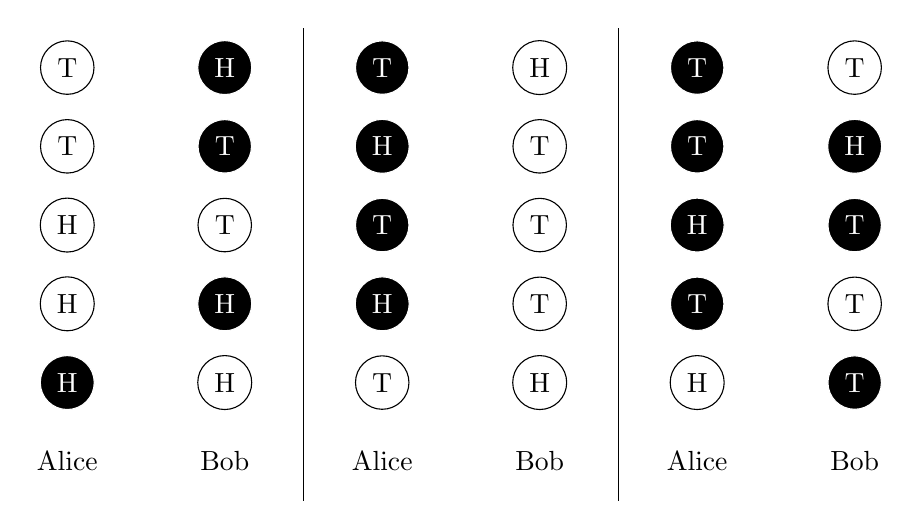
\begin{tikzpicture}
        \tikzmath{\rows = 5; \cols = 3; \intra = 2; \inter = 2; \rheight = 1;
        \nrowv = \rheight+\rheight; \theight = \rows*\rheight; 
        \colm = \cols-1; \ncolh = \inter+\intra; \twidth = \colm*\inter+\cols*\intra;}
        \draw (0,0) node {Alice} ++(\intra,0) node {Bob} ++(\inter,0) node {Alice} ++(\intra,0) node {Bob} ++(\inter,0) node {Alice} ++(\intra,0) node {Bob};
        \foreach \v in {\rheight,\nrowv,...,\theight} {
          \foreach \h in {0,\ncolh,...,\twidth} {
            \tikzmath{int \a, \b, \x, \y;
              \a = random(0,1); \b = random(0,1); \x = random(0,1); \y = random(0,1);
              if \a == 1 then { let \aval = H; } else { let \aval = T; };
              if \b == 1 then { let \bval = H; } else { let \bval = T; };
              if \x == 1 then { let \afg = black; let \abg = white; } else { let \afg = white; let \abg = black; };
              if \y == 1 then { let \bfg = black; let \bbg = white; } else { let \bfg = white; let \bbg = black; };
            }

            % TODO DOES NOT WORK
            % \draw (\h, \v) node[coin={bg = \abg, fg = \afg}] {\aval} ++(\intra,0) node[coin={bg = \bbg, fg = \bfg}] {\bval};
            \draw (\h, \v) node[circle,draw=\afg, text=\afg, fill=\abg,] {\aval} ++(\intra,0) node[circle,draw=\bfg, text=\bfg, fill=\bbg, ] {\bval}; 
          }
        }

        \tikzmath{\ilineh = \intra+0.5*\inter; \nlineh = \ilineh+\intra+\inter;}
        \foreach \h in {\ilineh, \nlineh} {
          \path[draw=black] (\h, -0.5*\rheight) -- (\h, \theight+0.5*\rheight);
        }
      \end{tikzpicture}
      \caption{Uncorrelated statistics}%
    \end{figure}
  \end{onlyenv}

  \begin{onlyenv}<2>
    \begin{figure}
      \centering
      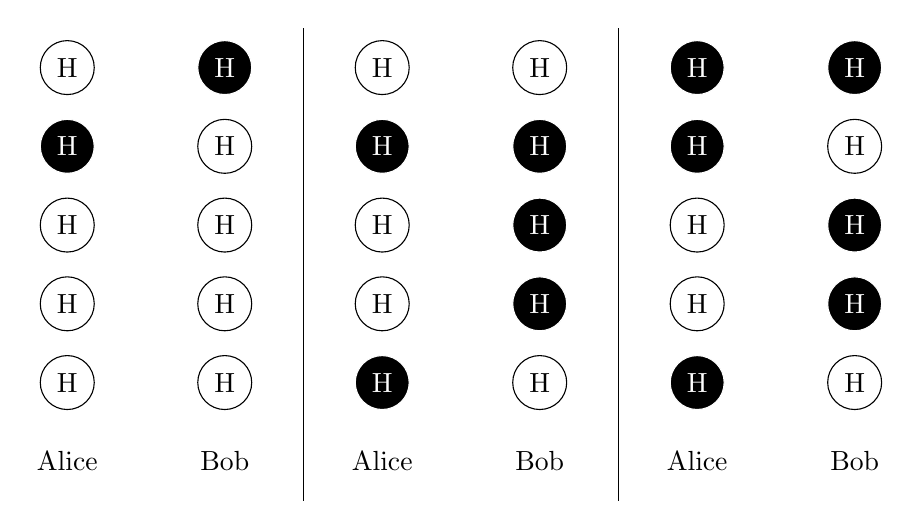
\begin{tikzpicture}
        \tikzmath{\rows = 5; \cols = 3; \intra = 2; \inter = 2; \rheight = 1;
        \nrowv = \rheight+\rheight; \theight = \rows*\rheight; 
        \colm = \cols-1; \ncolh = \inter+\intra; \twidth = \colm*\inter+\cols*\intra;}
        \draw (0,0) node {Alice} ++(\intra,0) node {Bob} ++(\inter,0) node {Alice} ++(\intra,0) node {Bob} ++(\inter,0) node {Alice} ++(\intra,0) node {Bob};
        \foreach \v in {\rheight,\nrowv,...,\theight} {
          \foreach \h in {0,\ncolh,...,\twidth} {
            \tikzmath{int \a, \b, \x, \y;
              \x = random(0,1); \y = random(0,1);
              if \x == 1 then { let \afg = black; let \abg = white; } else { let \afg = white; let \abg = black; };
              if \y == 1 then { let \bfg = black; let \bbg = white; } else { let \bfg = white; let \bbg = black; };
            }

            \draw (\h, \v) node[circle,draw=\afg, text=\afg, fill=\abg,] {H} ++(\intra,0) node[circle,draw=\bfg, text=\bfg, fill=\bbg, ] {H}; 
          }
        }

        \tikzmath{\ilineh = \intra+0.5*\inter; \nlineh = \ilineh+\intra+\inter;}
        \foreach \h in {\ilineh, \nlineh} {
          \path[draw=black] (\h, -0.5*\rheight) -- (\h, \theight+0.5*\rheight);
        }
      \end{tikzpicture}
      \caption{Locally correlated statistics}%
    \end{figure}
  \end{onlyenv}

  \begin{onlyenv}<3>
    \begin{figure}
      \centering
      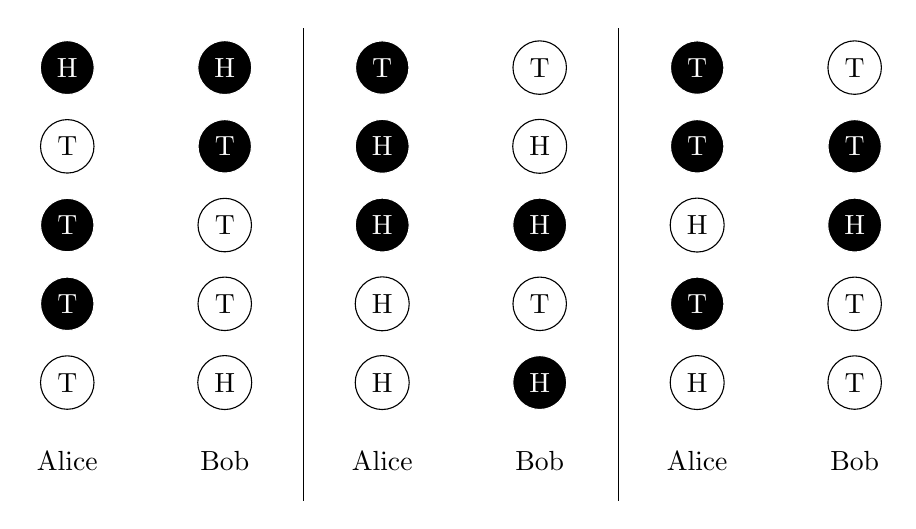
\begin{tikzpicture}
        \tikzmath{\rows = 5; \cols = 3; \intra = 2; \inter = 2; \rheight = 1;
        \nrowv = \rheight+\rheight; \theight = \rows*\rheight; 
        \colm = \cols-1; \ncolh = \inter+\intra; \twidth = \colm*\inter+\cols*\intra;}
        \draw (0,0) node {Alice} ++(\intra,0) node {Bob} ++(\inter,0) node {Alice} ++(\intra,0) node {Bob} ++(\inter,0) node {Alice} ++(\intra,0) node {Bob};
        \foreach \v in {\rheight,\nrowv,...,\theight} {
          \foreach \h in {0,\ncolh,...,\twidth} {
            \tikzmath{int \a, \b, \x, \y;
              \x = random(0,1); \y = random(0,1); \o = random(0,1);
              if \o == 1 then { let \aval = H; let \bval = T; } else { let \aval = T; let \bval = H; };
              if \x == 1 then { let \afg = black; let \abg = white; } else { let \afg = white; let \abg = black; };
              if \y == 1 then { let \bfg = black; let \bbg = white; } else { let \bfg = white; let \bbg = black; };
              if \x * \y != 1 then { let \bval = \aval; };
            }

            \draw (\h, \v) node[circle,draw=\afg, text=\afg, fill=\abg,] {\aval} ++(\intra,0) node[circle,draw=\bfg, text=\bfg, fill=\bbg, ] {\bval}; 
          }
        }

        \tikzmath{\ilineh = \intra+0.5*\inter; \nlineh = \ilineh+\intra+\inter;}
        \foreach \h in {\ilineh, \nlineh} {
          \path[draw=black] (\h, -0.5*\rheight) -- (\h, \theight+0.5*\rheight);
        }
      \end{tikzpicture}
      \caption{Nonlocally correlated statistics}%
    \end{figure}
  \end{onlyenv}
\end{frame}

\note{ Alice and Bob each have a jar of black coins and a jar of white coins. They play a game where, in each round, they take a coin from each jar, choose one coin, and flip it. }

\begin{frame}{Nonlocal Statistics}
  \begin{itemize}[<+->]
    \item Alice: input \(x\), output \(a\); Bob: input \(y\), output \(b\)
    \item Full statistics: \emph{behaviour} \(p(ab|xy)\) (aka \emph{state}/\emph{box})
    \item Must fulfill \emph{no-signalling conditions}
      \begin{gather*}
        \sum_b p(ab|xy) = p(a|xy) = p(a|x)\;\forall a,x,y \\
        \sum_a p(ab|xy) = p(b|xy) = p(b|y)\;\forall b,x,y
      \end{gather*}
    \item \emph{Setting}: \((i_A, o_A; i_B, o_B)\)
      \[ x \in \dintv{1}{i_A} \qquad a \in \dintv{1}{o_A} \]
      \[ y \in \dintv{1}{i_B} \qquad b \in \dintv{1}{o_B} \]
  \end{itemize}
\end{frame}

\begin{frame}{Nonlocal Behaviours}
  \begin{itemize}[<+->]
    \item \emph{Local set} \(\Ls\): \(p(ab|xy) = \int P_{\Lambda}(\lambda) p_{\lambda}(a|x)p_{\lambda}(b|y) \dif{\lambda} \)
    \item \emph{Quantum set} \(\Qs\): \(p(ab|xy) = \Tr{ \rho_{AB} \left(M_{a|x} \otimes N_{b|y}\right) }\)
    \item \emph{No-signalling set} \(\NSs\) defined by no-signalling conditions
    \item \(\Ls \subsetneq \Qs \subsetneq \NSs\)
  \end{itemize}
\end{frame}

\subsection{DIQKD}

\begin{frame}{Device Independent Security}
  \begin{itemize}[<+->]
    \item Consider
      \[ p(ab|xy) = \sum_e p_E(e) p_e(ab|xy) \]
    \item Eve can deduce \((a,b)\) from \((x,y)\) if \(p_e\)'s are \emph{deterministic}
    \item This is precisely \(\Ls\)
    \item Quantum processes provide \alert{fundamental indeterminism}
  \end{itemize}
\end{frame}

\note{ The following argument gives an intuition for the security of DIQKD\@. }

\begin{frame}{DIQKD Assumptions}
  \begin{itemize}[<+->]
        \item \emph{Sealed laboratories}: information transmission is controlled
        \item \emph{Trusted local randomness}: for generating inputs
        \item \emph{Authenticated classical channel}: distinct from \emph{confidentiality}
        \item \emph{Correctness} of quantum physics: for validity of proofs
  \end{itemize}
\end{frame}

\begin{frame}{DIQKD Security}
  \begin{itemize}[<+->]
    \item \(\rho_{\crv{A}^n\crv{X}^n \crv{B}^n\crv{Y}^n E^n}\): Alice--Bob--Eve ccq state after \(n\) Bell tests
          \[ \sum_{\cvec{a}^n\cvec{b}^n \cvec{x}^n\cvec{y}^n} \begin{aligned}[c]
          & \prin^n(\cvec{x}^n,\cvec{y}^n) p^n(\cvec{a}^n\cvec{b}^n|\cvec{x}^n\cvec{y}^n) \proj[\crv{A}^n\crv{X}^n \crv{B}^n\crv{Y}^n]{\cvec{a}^n\cvec{b}^n\cvec{x}^n\cvec{y}^n} \\
            \otimes & \rho_{E^n|\cvec{a}^n\cvec{x}^n \cvec{b}^n\cvec{y}^n}
          \end{aligned} \]
    \item \emph{Asymptotic key rate} of a sequence of states \(\{\rho^n\}\)
      \[ r(\proto{P}, \{\rho^n\}) = \lim_{n\to\infty} \frac{\ell_n - L_{\Omega}(\prin^n)}{n} \]
      if \emph{trace distance} from ideal final state is asymptotically vanishing
    \item \(L_{\Omega}(\prin^n)\): minimum cost for generating \(\prin^n\) (\alert{novel definition})
    \item Upper bounded by \emph{Wyner common information} if iid
    \item Dependent on protocol in general
  \end{itemize}
\end{frame}
\note{ \(\prin^n\) is typically assumed to be independent but we want to probe fundamental limits. Dependent inputs can avoid sifting factor (though this is multiplicative, not additive). This constrains the possible \(\prin^n\), since it must be generated with asymptotically zero error, or else the error needs to be accounted for in some other way. Protocols may allow recovery of input secrecy, so \(L_{\Omega}\) may be zero for dependent inputs. }

\begin{frame}{Security from Behaviours}
    \begin{itemize}[<+->]
      \item Optimise over \emph{states compatible with classical data} \(\compatstates[^n]{p}{\prin[\hat{p}^n]}\)
        \begin{itemize}
          \item Generated by valid qqq states and measurements
          \item Average behaviour matches \(p\)
          \item Input distribution is \(\prin[\hat{p}^n]\)
        \end{itemize}
      \item Well-established methods for reducing to iid
      \item Focus on \emph{iid secret key capacity}
        \[ C_{\sk}^{\otimes}(p) = \sup_{\proto{P}} \sup_{\prin} \inf_{\substack{\rho : \\ \rho \in \compatstates{p}{\prin}}} r(\proto{P}, \{\rho^{\otimes{n}}\}) \]
    \end{itemize}
\end{frame}

\section{Wirings}

\subsection{Wiring Distributions}

\begin{frame}{Local Operations and Shared Randomness}
  \begin{onlyenv}<1-3>
    \begin{itemize}[<+->]
      \item Take overall input, generate physical input, generate overall output from physical output
        \[ p'(a|x) = \sum_{a_0 x_0} p_o(a|x_0 a_0 x) p(a_0|x_0) p_i(x_0|x) \]
      \item Combine into a map obeying \emph{no-retrocausation}
        \[ \chi(a x_0 | x a_0) \coloneqq p_o(a|x_0a_0x) p_i(x_0|x) = p_o(a|x_0a_0x) p_i(x_0|x a_0) \]
      \item Combine with other party using \emph{shared randomness}
        \[ \chi(abx_0y_0|a_0b_0xy) \coloneqq \sum_{\lambda} P_{\Lambda}(\lambda) \chi_{A|\lambda}(ax_0|a_0x) \chi_{B|\lambda}(by_0|b_0y) \]
    \end{itemize}
  \end{onlyenv}
  \begin{onlyenv}<4->
    \begin{columns}
      \begin{column}[c]{0.3\linewidth}
        \centering
        \includegraphics{behav.tikz}
      \end{column}
      \begin{column}[c]{0.7\linewidth}
        \centering
        \includegraphics{losr.tikz}
      \end{column}
    \end{columns}
  \end{onlyenv}
\end{frame}

\begin{frame}{Wirings}
  \begin{onlyenv}<1-2>
    \begin{itemize}[<+->]
      \item Generalise to multiple boxes
        \begin{align*}
          p'(ab|xy) &\coloneqq \sum_{\cvec{a}^c\cvec{b}^c\cvec{x}^c\cvec{y}^c} \chi(ab\cvec{x}^c\cvec{y}^c|\cvec{a}^c\cvec{b}^cxy) p^c(\cvec{a}^c\cvec{b}^c|\cvec{x}^c\cvec{y}^c)\label{eqn:jwirdistdef} \\
          \chi(ab\cvec{x}^c\cvec{y}^c|\cvec{a}^c\cvec{b}^cxy) &\coloneqq \sum_{\lambda} P_{\Lambda}(\lambda) \chi_{A|\lambda}(a\cvec{x}^c|\cvec{a}^cx) \chi_{B|\lambda}(b\cvec{y}^c|\cvec{b}^cy) \\
          \chi_{A|\lambda}(\cvec{x}^j|\cvec{a}^cx) &= \chi_{A|\lambda}(\cvec{x}^j|\cvec{a}^{j-1}x),\,\forall j \in \dintv{1}{c} \\
          \chi_{B|\lambda}(\cvec{y}^j|\cvec{b}^cy) &= \chi_{B|\lambda}(\cvec{y}^j|\cvec{b}^{j-1}y),\,\forall j \in \dintv{1}{c}
        \end{align*}
      \item \emph{Marginal wirings} are sequences of stochastic maps
        \[ \chi_{A|\lambda}(a\cvec{x}^c|\cvec{a}^cx) = \chi_{A|\lambda}(a|\cvec{x}^c\cvec{a}^{c}x) \prod_{j=1}^c \chi_{A|\lambda}(x_j|\cvec{x}^{j-1}\cvec{a}^{j-1}x) \]
    \end{itemize}
  \end{onlyenv}
  \begin{onlyenv}<3->
    \begin{center}
      \includegraphics[height=0.85\textheight]{wiring.tikz}
    \end{center}
  \end{onlyenv}
\end{frame}

\begin{frame}{Structure of the Space of Wirings}
  \begin{itemize}[<+->]
    \item In each round, \emph{some} deterministic process has to be executed
      \begin{theorem}[Fine's Theorem for Wirings]
        The set of marginal wirings \(\sW\) forms a polytope, whose vertices are the set of deterministic marginal wirings obeying the no-retrocausation relations \(\sW_D\). All \(n\)-partite wirings are then elements of the polytope generated by the vertices \(\sW_D^n\).
      \end{theorem}
    \item Recursively split non-deterministic marginal wirings into probabilistic mixtures of deterministic ones
    \item Offload mixing into shared randomness
  \end{itemize}
\end{frame}

\subsection{Computational Descriptions}

\begin{frame}{Wiring Functions}
  \begin{itemize}[<+->]
    \item Objective: reduce no.\ of extremal wirings
    \item Deterministic maps are functions
    \item Combinatorics of sources and targets gives
      \[ \exp_{o_A}(i_A^c o_A^c) \prod_{j=1}^c \exp_{i_A}(i_A^{j} o_A^{j-1}) \]
      deterministic wirings
    \item Expressing as Karnaugh maps reveals redundancy, reduces to
      \[ \exp_{o_A}(i_A o_A^c) \prod_{j=1}^c \exp_{i_A}(i_A o_A^{j-1}) \]
  \end{itemize}
\end{frame}

\begin{frame}{Wiring Matrices}
  \begin{itemize}[<+->]
    \item Wirings permute sources (\(S\)), then map to targets (\(R\)), then permute targets (\(T\))
      \[ T_{c+1}R_{c+1}S_{c+1} \cdots T_2R_2S_2 T_1R_1S_1 p \]
    \item We can combine \(T_j\) and \(S_{j+1}\) if iterating over possible wirings
    \item Express each transformation as a matrix and multiply them together
    \item Easily extendable to \(n\)-partite wirings\only<.->{\footnote{If your computer has enough RAM}}
    \item Implemented and used to experiment with possible wirings
    \item Unfortunately gives the exact same number of wirings
  \end{itemize}
\end{frame}

\subsection{A Proposed Classification}

\begin{frame}{Couplers}
  \begin{itemize}[<+->]
    \item \emph{Couplers} map \(P(\cvec{a\breve{b}b}|\cvec{x\breve{y}y}) \mapsto P'(\cvec{a\breve{b}}b'|\cvec{x\breve{y}})\)
    \[ P'(\cvec{a\breve{b}}b'|\cvec{x\breve{y}}) = \sum_{\cvec{by}} \chi(b',\cvec{by})P(\cvec{a\breve{b}b}|\cvec{x\breve{y}y}) \]
    \item Polytope found by checking consistency of couplers on \(P(\cvec{b}|\cvec{y}) \in \NSs\)
    \item Wiring for a specific input: \emph{marginal conditional wiring distribution} (\(\chi_{A|\lambda}(a\cvec{x}^c|\cvec{a}^cx)\) for a given \(x\))
    \item \(\#\text{ couplers} < \#\text{ marginal conditional wiring distributions!}\)
    \item Could this simplify the space of wirings?
  \end{itemize}
\end{frame}

\begin{frame}{Number of Extremal Wirings}
  \begin{table}
    \begin{Tabular}{ccc} 
      \toprule
      Method & \(i = 2\) & \(i = 3\) \\
      \midrule
      Consistency on \(\NSs\) & \(82\), \(48\)  & --, \(2816\) \\
      Consistency on general behaviours & \(58\), \(512\) & --, \(524288\) \\
      Causal constraints & \(128\), -- & \(432\), -- \\
      \bottomrule
    \end{Tabular}
    \caption{Number of extremal wirings and facets}
  \end{table}
\end{frame}

\begin{frame}{Discussion}
  \begin{itemize}[<+->]
    \item Polytope for general behaviours contained within polytope for \(\NSs\)
    \item But wirings should not care about what they act on
    \item Hypothesis: signalling makes it impossible to implement certain transformations independently
    \item Connection to complete positivity of LOSR transformations?
    \item May be fruitful to analyse our own definitions for wirings
  \end{itemize}
\end{frame}

\section{Key Rates}

\subsection{Wirings without Output Dependency}

\begin{frame}{Simple Wirings Cannot Help}
  \begin{lemma}
    Define a \emph{wiring without output dependency} as a wiring for which all inputs are independent of previous outputs, that is, a wiring \(\chi\) that obeys
    \[
      \chi(\cvec{x}^c\cvec{y}^c|\cvec{a}^c\cvec{b}^cxy) = \chi(\cvec{x}^c\cvec{y}^c|xy).
    \]
    Make the weak assumption that operations that do not broadcast or discard information about the inputs will not impact the net cost of generating the input distribution. Then, any wiring with output dependency cannot increase the secret key capacity of a behaviour. That is, if \(p' = \chi[p]\), where \(\chi\) is a wiring without output dependency, then \(C_{\sk}^{\otimes}(p') \leq C_{\sk}^{\otimes}(p)\).
  \end{lemma}
\end{frame}

\begin{frame}{Proof Sketch}
  \begin{onlyenv}<1-3>
    \begin{itemize}[<+->]
      \item Wirings without output dependency obey
        \[ \chi(\cvec{x}^c\cvec{y}^c|xy) = \sum_{\lambda} P_{\Lambda}(\lambda) \chi_{A|\lambda}(\cvec{x}^c|x) \chi_{B|\lambda}(\cvec{y}^c|y) \]
      \item Measurements can generate \(\cvec{x}^c\) and \(\cvec{y}^c\) beforehand
      \item Can use same physical processes for \(p\) and \(p'\)
    \end{itemize}
  \end{onlyenv}
  \begin{onlyenv}<4-7> % TODO KIV removal
    \begin{itemize}[<+->]
      \item Quantum behaviour given by
        \[ p^c(\cvec{a}^c\cvec{b}^c|\cvec{x}^c\cvec{y}^c) = \Tr{\rho_{AB} \left( M_{\cvec{a}^c|\cvec{x}^c} \otimes N_{\cvec{b}^c|\cvec{y}^c} \right) } \]
      \item Wired behaviour given by
        \[ p'(ab|xy) = \sum_{\cvec{a}^c\cvec{b}^c\cvec{x}^c\cvec{y}^c} \sum_{\lambda} \begin{aligned}[c]
        & \chi_{A|\lambda}(a\cvec{x}^c|\cvec{a}^cx) \chi_{B|\lambda}(b\cvec{y}^c|\cvec{b}^cy) \\
        & P_{\Lambda}(\lambda) p^c(\cvec{a}^c\cvec{b}^c|\cvec{x}^c\cvec{y}^c)
        \end{aligned} \]
      \item Define \(M'_{a|x\lambda} \coloneqq \sum_{\cvec{a}^c\cvec{x}^c} \chi_{A|\lambda}(a\cvec{x}^c|\cvec{a}^cx) M_{\cvec{a}^c|\cvec{x}^c}\)
      \item These form a valid POVM with the same behaviour
        \[ \begin{aligned}[c]
          \sum_a M'_{a|x\lambda} &= \sum_a \sum_{\cvec{a}^c\cvec{x}^c} \chi_{A|\lambda}(a\cvec{x}^c|\cvec{a}^cx) M_{\cvec{a}^c|\cvec{x}^c} = \sum_{\cvec{a}^c\cvec{x}^c} \chi_{A|\lambda}(\cvec{x}^c|x) M_{\cvec{a}^c|\cvec{x}^c} \\
                                 &= \sum_{\cvec{x}^c} \chi_{A|\lambda}(\cvec{x}^c|x) I = I. \end{aligned} \]
    \end{itemize}
  \end{onlyenv}
  \begin{onlyenv}<8->
    \begin{center}
      \includegraphics[height=0.85\textheight]{outdep.tikz}
    \end{center}
  \end{onlyenv}
\end{frame}

\begin{frame}{Discussion}
  \begin{itemize}[<+->]
    \item Can generalise the argument about simulating the transformed statistics to other transformations
    \item AND wiring is a wiring without output dependency \(\Rightarrow\) no increase in capacity
    \item Private local randomness would be better used in noisy preprocessing
    \item Private shared randomness: \alert{still open}
    \item Possible connection to \emph{measurement dependence}
  \end{itemize}
\end{frame}

\subsection{Optimising over Wirings}

\begin{frame}{Key Rates of Extremal Wirings}
  \begin{onlyenv}<1-3>
    \begin{itemize}[<+->]
      \item \emph{Wired} secret key capacity:
        \[ C^{W}_{\sk}(p) \coloneqq \sup_{\chi\in\sW^2} C^{\otimes}_{\sk}(\chi[p]) \]
        \begin{theorem}
          The secret key capacity is convex, and therefore the wired secret key capacity is maximised by extremal wirings.
        \end{theorem}
      \item Standard convexity argument: Eve can use a probabilistic mixture of implementations, and the capacity of the mixture cannot exceed the mixture of the capacities
    \end{itemize}
  \end{onlyenv}
  \begin{onlyenv}<4-6>
    \begin{itemize}[<+->]
      \item Brute force search possible, but unclear how capacity changes with \(c\)
      \item Possible simplifications using techniques from dynamic or linear programming
      \item Caveat: bounds on capacity may not be convex
    \end{itemize}
  \end{onlyenv}
\end{frame}

% TODO KIV removal
\begin{frame}{Semidefinite Programming}
  \begin{itemize}[<+->]
    \item Computable lower bound of the form
      \[ C^{\otimes}_{\sk}(p) \geq c_m(1) + \inf_{\matr{M}\in\sM} Q_{m,k}(p, \matr{M}) - H{(\crv{A}|\crv{B})}_{p} \]
    \item Insert into definition of \(C_{\sk}^W\)
      \[ C^{W}_{\sk}(p) \geq \sup_{\chi\in\sW^2} \left[ c_m(1) + \inf_{\matr{M}\in\sM} Q_{m,k}(\chi[p], \matr{M}) - H{(\crv{A}|\crv{B})}_{\chi[p]} \right] \]
    \item \emph{Bilevel optimisation} (sup of inf): lower bound by replacing inner optimisation with dual
      \[ C^{W}_{\sk}(p) \geq \sup_{\chi\in\sW^2} \left[ c_m(1) + \sup_{\cvec{\mu} \in \sM'} Q'_{m,k}(\cvec{\mu}, \chi[p]) - H{(\crv{A}|\crv{B})}_{\chi[p]} \right] \]
    \item Unfortunately, dual objective function contains nonconvex terms
  \end{itemize}
\end{frame}

% TODO KIV removal
\subsection{Other Bounds}

\begin{frame}{Wiring Monotones}
  \begin{itemize}[<+->]
    \item Computable functions that are \emph{monotone} under wiring
    \item Only one so far: \emph{maximal correlation for wirings} \(\varrho\)
    \item Caveat: only for wirings without shared randomness
    \item Key rates maximised by deterministic wirings anyway
    \item Therefore, upper bound on \(C_{\sk}^{\otimes}\) of behaviours below a certain \(\varrho\) is an upper bound on \(C_{\sk}^W\)
  \end{itemize}
\end{frame}

\begin{frame}{Classical Upper Bounds}
  \begin{itemize}[<+->]
    \item Secret key rate from classical correlations is an upper bound
    \item A computable(ish) upper bound:
          \[ S(\crv{V}_1, \crv{V}_2||\crv{E}) \leq \inf_\crv{J} I(\crv{V}_1 : \crv{V}_2|\crv{J}) + I(\crv{V}_1\crv{V}_2 : \crv{J}|\crv{E}) \]
    \item Parametrised dimension-bounded correlations using paramterisation for unitaries
    \item Expressed objective function as polynomial/rational function using \emph{Gauss-Radau quadrature} and \emph{quasi-relative entropies}
    \item Explored global bounds on objective functions through SDPs
    \item Parameter space seems very large; may have to use Monte Carlo methods
  \end{itemize}
\end{frame}

\section*{Summary and Outlook}

\begin{frame}{DIQKD}
  \begin{itemize}[<+->]
    \item Proposed new key rate definition dependent on input distribution
    \item Proposed definition of secret key capacity in terms of all available classical data
  \end{itemize}
\end{frame}

\begin{frame}{Behaviours}
  \begin{itemize}[<+->]
    \item Wirings generalise local operations and shared randomness
    \item Convex hull of deterministic wirings
    \item Implemented computational representation
    \item Next step: investigate connection to couplers and measurement dependence
  \end{itemize}
\end{frame}

\begin{frame}{Key Rates}
  \begin{itemize}[<+->]
    \item Maximised by extremal wirings
    \item BFF method gives nonconvex optimisation
    \item Maximal correlation provides valid upper bounds, but further utility unclear
    \item Some preliminary work in establishing computationally tractable bounds
  \end{itemize}
\end{frame}

\begin{frame}[c]{}
  \begin{center}
    \begin{beamercolorbox}[sep=8pt,center,shadow=true,rounded=true]{title}
      Thank you!
    \end{beamercolorbox}
  \end{center}
\end{frame}

% Placing a * after \section means it will not show in the
% outline or table of contents.

\end{document}

